\documentclass{article}\usepackage[]{graphicx}\usepackage[]{color}
%% maxwidth is the original width if it is less than linewidth
%% otherwise use linewidth (to make sure the graphics do not exceed the margin)
\makeatletter
\def\maxwidth{ %
  \ifdim\Gin@nat@width>\linewidth
    \linewidth
  \else
    \Gin@nat@width
  \fi
}
\makeatother

\definecolor{fgcolor}{rgb}{0.345, 0.345, 0.345}
\newcommand{\hlnum}[1]{\textcolor[rgb]{0.686,0.059,0.569}{#1}}%
\newcommand{\hlstr}[1]{\textcolor[rgb]{0.192,0.494,0.8}{#1}}%
\newcommand{\hlcom}[1]{\textcolor[rgb]{0.678,0.584,0.686}{\textit{#1}}}%
\newcommand{\hlopt}[1]{\textcolor[rgb]{0,0,0}{#1}}%
\newcommand{\hlstd}[1]{\textcolor[rgb]{0.345,0.345,0.345}{#1}}%
\newcommand{\hlkwa}[1]{\textcolor[rgb]{0.161,0.373,0.58}{\textbf{#1}}}%
\newcommand{\hlkwb}[1]{\textcolor[rgb]{0.69,0.353,0.396}{#1}}%
\newcommand{\hlkwc}[1]{\textcolor[rgb]{0.333,0.667,0.333}{#1}}%
\newcommand{\hlkwd}[1]{\textcolor[rgb]{0.737,0.353,0.396}{\textbf{#1}}}%

\usepackage{framed}
\makeatletter
\newenvironment{kframe}{%
 \def\at@end@of@kframe{}%
 \ifinner\ifhmode%
  \def\at@end@of@kframe{\end{minipage}}%
  \begin{minipage}{\columnwidth}%
 \fi\fi%
 \def\FrameCommand##1{\hskip\@totalleftmargin \hskip-\fboxsep
 \colorbox{shadecolor}{##1}\hskip-\fboxsep
     % There is no \\@totalrightmargin, so:
     \hskip-\linewidth \hskip-\@totalleftmargin \hskip\columnwidth}%
 \MakeFramed {\advance\hsize-\width
   \@totalleftmargin\z@ \linewidth\hsize
   \@setminipage}}%
 {\par\unskip\endMakeFramed%
 \at@end@of@kframe}
\makeatother

\definecolor{shadecolor}{rgb}{.97, .97, .97}
\definecolor{messagecolor}{rgb}{0, 0, 0}
\definecolor{warningcolor}{rgb}{1, 0, 1}
\definecolor{errorcolor}{rgb}{1, 0, 0}
\newenvironment{knitrout}{}{} % an empty environment to be redefined in TeX

\usepackage{alltt}

\usepackage{comment}
\usepackage[english]{isodate}

\usepackage{graphicx}
\usepackage{siunitx}
\usepackage{paracol}
\usepackage{amsmath}
\usepackage{ amssymb }
\usepackage[utf8]{inputenc}

\usepackage{mathtools,xparse}

\DeclarePairedDelimiter{\abs}{\lvert}{\rvert}
\DeclarePairedDelimiter{\norm}{\lVert}{\rVert}

\newcommand{\E}{\mathrm{E}}
\newcommand{\Var}{\mathrm{Var}}
\newcommand{\Cov}{\mathrm{Cov}}



\sisetup{output-decimal-marker = {,}}
\newcommand*{\ft}[1]{_\mathrm{#1}} 
\newcommand*{\dd}{\mathop{}\!\mathrm{d}}
\newcommand*{\tran}{^{\mkern-1.5mu\mathsf{T}}}%transpose of matrix
\newcommand{\trace}{\mathrm{trace}}
\IfFileExists{upquote.sty}{\usepackage{upquote}}{}
\begin{document}

	\begin{titlepage}
		\begin{center}
			\vspace*{1cm}
			\textbf{Math 423}\\
			\text{Linear Regression}\\
			\vspace{0.5cm}
			Homework IV
			
			\vspace{1.5cm}
			
			\textbf{Frédéric Boileau}\\
			\vspace{2cm}
			Prof. 
			David A. Stephens
			\vfill
			\today
			\thispagestyle{empty}
		\end{center}
	\end{titlepage}

\section*{1}
\subsection*{a}




\begin{knitrout}
\definecolor{shadecolor}{rgb}{0.969, 0.969, 0.969}\color{fgcolor}\begin{kframe}
\begin{alltt}
\hlkwd{setwd}\hlstd{(}\hlkwd{dirname}\hlstd{(rstudioapi}\hlopt{::}\hlkwd{getActiveDocumentContext}\hlstd{()}\hlopt{$}\hlstd{path))}
\end{alltt}


{\ttfamily\noindent\bfseries\color{errorcolor}{\#\# Error: RStudio not running}}\begin{alltt}
\hlstd{testScores} \hlkwb{=} \hlkwd{read.csv}\hlstd{(}\hlstr{"TestScores.csv"}\hlstd{,}\hlkwc{header}\hlstd{=}\hlnum{TRUE}\hlstd{)}
\hlstd{testScores}\hlopt{$}\hlstd{Faculty} \hlkwb{=} \hlkwd{as.factor}\hlstd{(testScores}\hlopt{$}\hlstd{Faculty)}
\hlstd{yT} \hlkwb{=} \hlstd{testScores}\hlopt{$}\hlstd{Score}
\hlstd{faculty} \hlkwb{=} \hlstd{testScores}\hlopt{$}\hlstd{Faculty}
\end{alltt}
\end{kframe}
\end{knitrout}



Now that we have converted the qualitative data's class into factors we can fit the model using lm. This is a model with only one predictor with three levels. Moreover we directly sum up the results in a boxplot to get an idea of the fit by quick inspection.

\begin{knitrout}
\definecolor{shadecolor}{rgb}{0.969, 0.969, 0.969}\color{fgcolor}\begin{kframe}
\begin{alltt}
\hlstd{fit.yT} \hlkwb{=} \hlkwd{lm}\hlstd{(yT} \hlopt{~} \hlstd{faculty)}
\hlstd{clrs} \hlkwb{=} \hlkwd{c}\hlstd{(}\hlstr{"red"}\hlstd{,} \hlstr{"blue"}\hlstd{,} \hlstr{"green"}\hlstd{)}
\hlkwd{boxplot}\hlstd{(}\hlkwd{residuals}\hlstd{(fit.yT)} \hlopt{~} \hlstd{faculty,} \hlkwc{vertical} \hlstd{=} \hlnum{TRUE}\hlstd{,} \hlkwc{col} \hlstd{= clrs)}
\end{alltt}
\end{kframe}
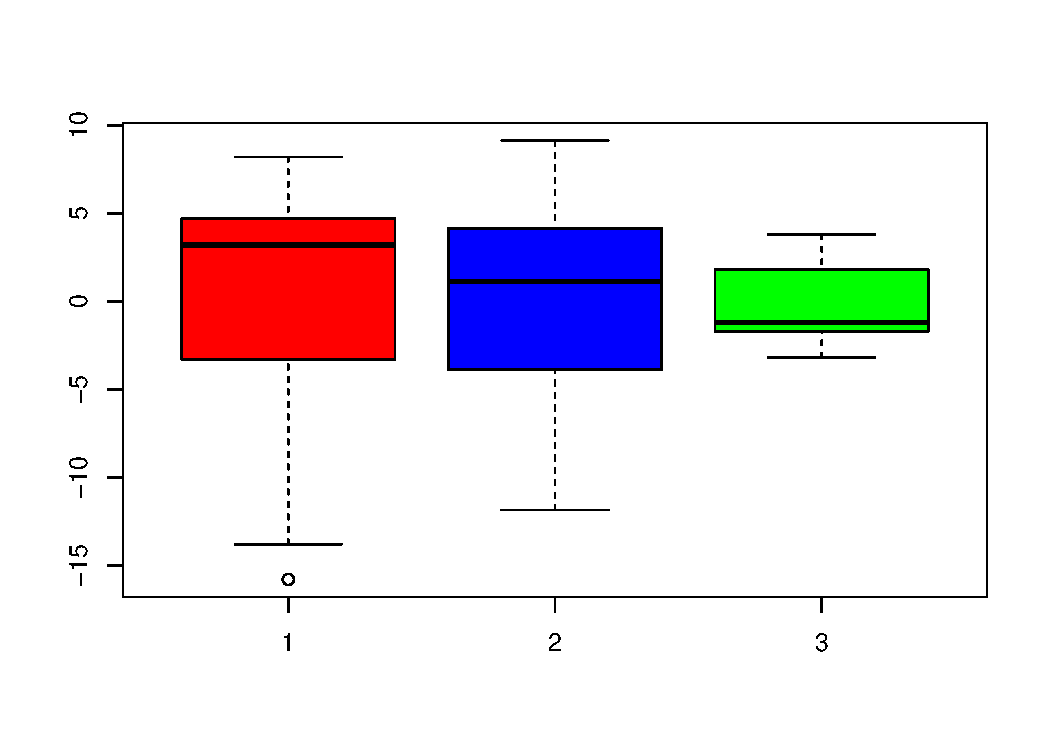
\includegraphics[width=\maxwidth]{figure/unnamed-chunk-2-1} 

\end{knitrout}



From the onset we see that there is a wide disparity of variance between the first two faculties and the third. This is especially true when compared with the means. To take at closer look at the situation let's run an anova

\begin{knitrout}
\definecolor{shadecolor}{rgb}{0.969, 0.969, 0.969}\color{fgcolor}\begin{kframe}
\begin{alltt}
\hlkwd{anova}\hlstd{(fit.yT)}
\end{alltt}
\begin{verbatim}
## Analysis of Variance Table
## 
## Response: yT
##           Df Sum Sq Mean Sq F value    Pr(>F)    
## faculty    2 1529.4  764.69  20.016 7.843e-07 ***
## Residuals 42 1604.5   38.20                      
## ---
## Signif. codes:  0 '***' 0.001 '**' 0.01 '*' 0.05 '.' 0.1 ' ' 1
\end{verbatim}
\end{kframe}
\end{knitrout}
We get a very small p-value for the regression so we conclude there is a statistically significant difference between test score for students from the 3 different faculties. 

\begin{knitrout}
\definecolor{shadecolor}{rgb}{0.969, 0.969, 0.969}\color{fgcolor}\begin{kframe}
\begin{alltt}
\hlkwd{library}\hlstd{(lsmeans)}
\end{alltt}


{\ttfamily\noindent\color{warningcolor}{\#\# Warning: package 'lsmeans' was built under R version 3.3.2}}

{\ttfamily\noindent\itshape\color{messagecolor}{\#\# Loading required package: estimability}}

{\ttfamily\noindent\color{warningcolor}{\#\# Warning: package 'estimability' was built under R version 3.3.2}}\begin{alltt}
\hlstd{means.yT} \hlkwb{=} \hlkwd{lsmeans}\hlstd{(fit.yT,} \hlopt{~} \hlstd{faculty)}
\hlkwd{print}\hlstd{(means.yT)}
\end{alltt}
\begin{verbatim}
##  faculty   lsmean       SE df lower.CL upper.CL
##  1       35.80000 1.595894 42 32.57936 39.02064
##  2       35.86667 1.595894 42 32.64602 39.08731
##  3       48.20000 1.595894 42 44.97936 51.42064
## 
## Confidence level used: 0.95
\end{verbatim}
\end{kframe}
\end{knitrout}
The means of the test scores of students in differentiated by faculty and their respective standard
errors are displayed above. The means with their standard errors beeing in the second and third columns respectively.
\clearpage
\section*{2}
\subsection*{a}
As for the preceding section the first thing we do is import the data and format it appropriately
\begin{knitrout}
\definecolor{shadecolor}{rgb}{0.969, 0.969, 0.969}\color{fgcolor}\begin{kframe}
\begin{alltt}
\hlstd{filter} \hlkwb{=} \hlkwd{read.csv}\hlstd{(}\hlstr{"Filter.csv"}\hlstd{)}
\hlstd{filter}\hlopt{$}\hlstd{carsize} \hlkwb{=} \hlkwd{as.factor}\hlstd{(filter}\hlopt{$}\hlstd{carsize)}
\hlstd{filter}\hlopt{$}\hlstd{type} \hlkwb{=} \hlkwd{as.factor}\hlstd{(filter}\hlopt{$}\hlstd{type)}
\hlstd{yF} \hlkwb{=} \hlstd{filter}\hlopt{$}\hlstd{noise}
\hlstd{type} \hlkwb{=} \hlstd{filter}\hlopt{$}\hlstd{type}
\hlstd{carsize} \hlkwb{=} \hlstd{filter}\hlopt{$}\hlstd{carsize}
\end{alltt}
\end{kframe}
\end{knitrout}

Now we have 2 predictors and we want to fit the five possible models as liste in page 1. We have to type of predictors; factor predictors and interactions of factor predictors. Consequently interactions are counted as predictors in their own right. So a model with two predictors and their interaction has 4 parameters including the intercept. We now fit the 5 possible models 

\begin{knitrout}
\definecolor{shadecolor}{rgb}{0.969, 0.969, 0.969}\color{fgcolor}\begin{kframe}
\begin{alltt}
\hlstd{fit.nothing} \hlkwb{=} \hlkwd{lm}\hlstd{(yF} \hlopt{~} \hlnum{1}\hlstd{)}
\hlstd{fit.carsize} \hlkwb{=} \hlkwd{lm}\hlstd{(yF} \hlopt{~} \hlstd{carsize,} \hlkwc{data} \hlstd{= filter)}
\hlstd{fit.type} \hlkwb{=} \hlkwd{lm}\hlstd{(yF} \hlopt{~} \hlstd{type)}
\hlstd{fit.both} \hlkwb{=} \hlkwd{lm}\hlstd{(yF} \hlopt{~} \hlstd{carsize} \hlopt{+} \hlstd{type)}
\hlstd{fit.interaction} \hlkwb{=} \hlkwd{lm}\hlstd{(yF} \hlopt{~} \hlstd{carsize} \hlopt{+} \hlstd{type} \hlopt{+}\hlstd{carsize}\hlopt{:}\hlstd{type)}
\end{alltt}
\end{kframe}
\end{knitrout}
To have a table displaying the residual sum of squares of the 5 different models and the number of parameters for each model we can simply call the anova function with the models as arguments to get in one function call all the SSres.
\clearpage
\begin{knitrout}
\definecolor{shadecolor}{rgb}{0.969, 0.969, 0.969}\color{fgcolor}\begin{kframe}
\begin{alltt}
\hlstd{a.1} \hlkwb{=} \hlkwd{anova}\hlstd{(fit.nothing,fit.type, fit.carsize, fit.both, fit.interaction)}
\hlkwd{print}\hlstd{(a.1)}
\end{alltt}
\begin{verbatim}
## Analysis of Variance Table
## 
## Model 1: yF ~ 1
## Model 2: yF ~ type
## Model 3: yF ~ carsize
## Model 4: yF ~ carsize + type
## Model 5: yF ~ carsize + type + carsize:type
##   Res.Df     RSS Df Sum of Sq        F    Pr(>F)    
## 1     35 29874.3                                    
## 2     34 28818.1  1    1056.2  16.1465 0.0003631 ***
## 3     33  3822.9  1   24995.1 382.0913 < 2.2e-16 ***
## 4     32  2766.7  1    1056.2  16.1465 0.0003631 ***
## 5     30  1962.5  2     804.2   6.1465 0.0057915 ** 
## ---
## Signif. codes:  0 '***' 0.001 '**' 0.01 '*' 0.05 '.' 0.1 ' ' 1
\end{verbatim}
\end{kframe}
\end{knitrout}
\begin{table}[htbp!]
		\begin{center}
			\begin{tabular}{| c | c | c |}
			\hline Model & $SS_{res}$ & p	\\
			\hline 1 & \ensuremath{2.9874306\times 10^{4}}  & 1\\
			\hline 1 + type & \ensuremath{2.8818056\times 10^{4}} & 2\\
			\hline 1 + carsize & 3822.9166667 & 3\\
			\hline 1 + type + carsize & 2766.6666667 & 4\\
			\hline 1 + type + carsize + type*carsize & 1962.5& 6\\
			\hline	
			\end{tabular}
	\end{center}
\end{table}

\clearpage

\subsection*{b}
We now compare the "reduced" model which only considers the predictor "carsize" to the one that also includes the "type" predictor. When we include the main effect of a predictor we include all possible interactions as standard practice as to not make arbitrarily determined levels relevant (also vice-versa).
\begin{knitrout}
\definecolor{shadecolor}{rgb}{0.969, 0.969, 0.969}\color{fgcolor}\begin{kframe}
\begin{alltt}
\hlstd{a.2} \hlkwb{=} \hlkwd{anova}\hlstd{(fit.carsize,fit.interaction)}
\hlkwd{print}\hlstd{(a.2)}
\end{alltt}
\begin{verbatim}
## Analysis of Variance Table
## 
## Model 1: yF ~ carsize
## Model 2: yF ~ carsize + type + carsize:type
##   Res.Df    RSS Df Sum of Sq      F    Pr(>F)    
## 1     33 3822.9                                  
## 2     30 1962.5  3    1860.4 9.4798 0.0001461 ***
## ---
## Signif. codes:  0 '***' 0.001 '**' 0.01 '*' 0.05 '.' 0.1 ' ' 1
\end{verbatim}
\end{kframe}
\end{knitrout}
Now to compute manually the p value of the partial F test we need to determine the degrees of freedom of the numerator (r) and the denominator(n-p). For the full model we have to two type of parameters; $p_1 =M_{carsize} + M_{type} - 1 = 3 + 2 - 1 = 4$ for the main effects and $p_2 = (M_{carsize} -1) (M_{type} - 1) = 2$ for the interections. Adding up we get $p = p_1 + p_2 = 6$. The reduced model has one factor variable with 3 levels so 3 parameters. The difference in both is 3 so $r = 3$ and 
\begin{knitrout}
\definecolor{shadecolor}{rgb}{0.969, 0.969, 0.969}\color{fgcolor}\begin{kframe}
\begin{alltt}
\hlstd{r} \hlkwb{=} \hlnum{3}
\hlstd{n} \hlkwb{=} \hlnum{36}
\hlstd{p} \hlkwb{=} \hlnum{6}
\hlstd{df1} \hlkwb{=}\hlstd{r}
\hlstd{df2} \hlkwb{=} \hlstd{n}\hlopt{-}\hlstd{p}
\hlstd{num1} \hlkwb{=} \hlkwd{sum}\hlstd{(}\hlkwd{residuals}\hlstd{(fit.carsize)}\hlopt{^}\hlnum{2}\hlstd{)}\hlopt{/} \hlstd{df1}
\hlstd{num2} \hlkwb{=} \hlkwd{sum}\hlstd{(}\hlkwd{residuals}\hlstd{(fit.interaction)}\hlopt{^}\hlnum{2}\hlstd{)} \hlopt{/} \hlstd{df1}
\hlstd{num} \hlkwb{=} \hlstd{num1} \hlopt{-} \hlstd{num2}
\hlstd{den}\hlkwb{=}  \hlstd{(}\hlkwd{sum}\hlstd{(}\hlkwd{residuals}\hlstd{(fit.interaction)}\hlopt{^}\hlnum{2}\hlstd{)}\hlopt{/}\hlstd{(df2))}
\hlstd{f_stat} \hlkwb{=} \hlstd{num}\hlopt{/}\hlstd{den}
\hlstd{p_value} \hlkwb{=} \hlnum{1} \hlopt{-} \hlkwd{pf}\hlstd{(f_stat,df1,df2)}
\hlkwd{print}\hlstd{(f_stat)}
\end{alltt}
\begin{verbatim}
## [1] 9.47983
\end{verbatim}
\begin{alltt}
\hlkwd{print}\hlstd{(p_value)}
\end{alltt}
\begin{verbatim}
## [1] 0.0001460971
\end{verbatim}
\end{kframe}
\end{knitrout}

\clearpage

\section*{3}

To evaluate the effect of having surgery on patient satisfaction we have to also consider the rest of the data. We want to build an adequate model for patient satisfaction in a hospital. We have four possible predictors, all of them continuous except one; a factor predictor. The factor predictor has two levels indicating if the patient has had surgery or not. We start by looking at a full additive model
\begin{knitrout}
\definecolor{shadecolor}{rgb}{0.969, 0.969, 0.969}\color{fgcolor}\begin{kframe}
\begin{alltt}
\hlkwd{library}\hlstd{(car)}
\hlstd{pat} \hlkwb{=} \hlkwd{read.csv}\hlstd{(}\hlstr{"PatSat.csv"}\hlstd{,} \hlkwc{header} \hlstd{=} \hlnum{TRUE}\hlstd{)}
\hlstd{pat}\hlopt{$}\hlstd{Surgery} \hlkwb{=} \hlkwd{as.factor}\hlstd{(pat}\hlopt{$}\hlstd{Surgery)}
\hlstd{y} \hlkwb{=} \hlstd{pat}\hlopt{$}\hlstd{Satisfaction}
\hlstd{age} \hlkwb{=} \hlstd{pat}\hlopt{$}\hlstd{Age}
\hlstd{sev} \hlkwb{=} \hlstd{pat}\hlopt{$}\hlstd{Severity}
\hlstd{sur} \hlkwb{=} \hlstd{pat}\hlopt{$}\hlstd{Surgery}
\hlstd{anx} \hlkwb{=} \hlstd{pat}\hlopt{$}\hlstd{Anxiety}
\hlstd{fit.add} \hlkwb{=} \hlkwd{lm}\hlstd{(y} \hlopt{~} \hlstd{age} \hlopt{+} \hlstd{sev} \hlopt{+} \hlstd{sur} \hlopt{+} \hlstd{anx)}
\hlkwd{vif}\hlstd{(fit.add)}
\end{alltt}
\begin{verbatim}
##      age      sev      sur      anx 
## 1.939128 1.441055 1.072782 1.689768
\end{verbatim}
\end{kframe}
\end{knitrout}

\begin{knitrout}
\definecolor{shadecolor}{rgb}{0.969, 0.969, 0.969}\color{fgcolor}\begin{kframe}
\begin{alltt}
\hlkwd{summary}\hlstd{(fit.add)}
\end{alltt}
\begin{verbatim}
## 
## Call:
## lm(formula = y ~ age + sev + sur + anx)
## 
## Residuals:
##     Min      1Q  Median      3Q     Max 
## -18.506  -5.096   1.306   4.738  28.722 
## 
## Coefficients:
##             Estimate Std. Error t value Pr(>|t|)    
## (Intercept) 140.1689     8.3191  16.849 2.77e-13 ***
## age          -1.1428     0.1904  -6.002 7.22e-06 ***
## sev          -0.4699     0.1866  -2.518   0.0204 *  
## surYes        2.2259     4.1402   0.538   0.5968    
## anx           1.2673     1.4922   0.849   0.4058    
## ---
## Signif. codes:  0 '***' 0.001 '**' 0.01 '*' 0.05 '.' 0.1 ' ' 1
## 
## Residual standard error: 9.921 on 20 degrees of freedom
## Multiple R-squared:  0.8183,	Adjusted R-squared:  0.7819 
## F-statistic: 22.51 on 4 and 20 DF,  p-value: 3.611e-07
\end{verbatim}
\end{kframe}
\end{knitrout}
\clearpage
We achieve with this model a reasonable although not very high adjusted R-squared value. Now we want to scale back; the main effects of the variables Surgery and Anxiety appear to not be significant in this model before considering interactions. Moreoever we are lucky in that the predictor \textit surgery has a very low VIF  so multicollinearity will not be a major problem in evaluating if surgery affects patient satisfaction. We decide to start with a model containing only the main effects of age and severity.


\begin{knitrout}
\definecolor{shadecolor}{rgb}{0.969, 0.969, 0.969}\color{fgcolor}\begin{kframe}
\begin{alltt}
\hlstd{fit.ageSeverity} \hlkwb{=} \hlkwd{lm}\hlstd{(y} \hlopt{~} \hlstd{age} \hlopt{+} \hlstd{sev)}
\hlkwd{summary}\hlstd{(fit.ageSeverity)}
\end{alltt}
\begin{verbatim}
## 
## Call:
## lm(formula = y ~ age + sev)
## 
## Residuals:
##      Min       1Q   Median       3Q      Max 
## -18.3691  -5.9535   0.2975   4.0462  29.3439 
## 
## Coefficients:
##             Estimate Std. Error t value Pr(>|t|)    
## (Intercept) 139.9233     8.1002  17.274 2.78e-14 ***
## age          -1.0462     0.1573  -6.652 1.09e-06 ***
## sev          -0.4359     0.1788  -2.439   0.0233 *  
## ---
## Signif. codes:  0 '***' 0.001 '**' 0.01 '*' 0.05 '.' 0.1 ' ' 1
## 
## Residual standard error: 9.682 on 22 degrees of freedom
## Multiple R-squared:  0.8096,	Adjusted R-squared:  0.7923 
## F-statistic: 46.77 on 2 and 22 DF,  p-value: 1.193e-08
\end{verbatim}
\end{kframe}
\end{knitrout}
First we notice that our R-squared values has augmented though very midly while the standard R squared value is almost the same. We look for further simplification:
\begin{knitrout}
\definecolor{shadecolor}{rgb}{0.969, 0.969, 0.969}\color{fgcolor}\begin{kframe}
\begin{alltt}
\hlkwd{drop1}\hlstd{(fit.ageSeverity,} \hlkwc{test} \hlstd{=} \hlstr{"F"}\hlstd{)}
\end{alltt}
\begin{verbatim}
## Single term deletions
## 
## Model:
## y ~ age + sev
##        Df Sum of Sq    RSS    AIC F value    Pr(>F)    
## <none>              2062.3 116.32                      
## age     1    4148.3 6210.6 141.88 44.2528 1.092e-06 ***
## sev     1     557.4 2619.7 120.30  5.9467   0.02328 *  
## ---
## Signif. codes:  0 '***' 0.001 '**' 0.01 '*' 0.05 '.' 0.1 ' ' 1
\end{verbatim}
\end{kframe}
\end{knitrout}
The F-test indicates we cannot simplify this model further according to our choice of Fout (4)
We now look at possible interactions between the two predictors. We again follow the rule that all main effects have to be included whenever we consider interactions. 
\begin{knitrout}
\definecolor{shadecolor}{rgb}{0.969, 0.969, 0.969}\color{fgcolor}\begin{kframe}
\begin{alltt}
\hlstd{fit.ageSeverity_int} \hlkwb{=} \hlkwd{lm}\hlstd{(y} \hlopt{~} \hlstd{age} \hlopt{+} \hlstd{sev} \hlopt{+} \hlstd{age}\hlopt{:}\hlstd{sev)}
\hlkwd{anova}\hlstd{(fit.ageSeverity, fit.ageSeverity_int)}
\end{alltt}
\begin{verbatim}
## Analysis of Variance Table
## 
## Model 1: y ~ age + sev
## Model 2: y ~ age + sev + age:sev
##   Res.Df    RSS Df Sum of Sq      F Pr(>F)
## 1     22 2062.3                           
## 2     21 2032.7  1    29.549 0.3053 0.5864
\end{verbatim}
\end{kframe}
\end{knitrout}
We don't need any further analysis to see that the added interaction term doesn't add any statistical significane to the model.Nevertheless we want to look at all possible interactions of the second order and compare them. To the model that only considers the main effects of age and severity (the "best" one so far).
\clearpage
\begin{knitrout}
\definecolor{shadecolor}{rgb}{0.969, 0.969, 0.969}\color{fgcolor}\begin{kframe}
\begin{alltt}
\hlstd{fit.allSecond} \hlkwb{=} \hlkwd{lm}\hlstd{(y} \hlopt{~} \hlstd{age}\hlopt{*}\hlstd{(sev} \hlopt{+} \hlstd{anx} \hlopt{+} \hlstd{sur))}
\hlkwd{summary}\hlstd{(fit.allSecond)}
\end{alltt}
\begin{verbatim}
## 
## Call:
## lm(formula = y ~ age * (sev + anx + sur))
## 
## Residuals:
##     Min      1Q  Median      3Q     Max 
## -17.804  -5.544  -1.247   3.747  29.387 
## 
## Coefficients:
##               Estimate Std. Error t value Pr(>|t|)   
## (Intercept) 138.754434  44.705750   3.104  0.00645 **
## age          -1.119644   0.840185  -1.333  0.20025   
## sev          -0.122382   1.318898  -0.093  0.92715   
## anx          -3.473254  13.038771  -0.266  0.79315   
## surYes        9.850133  20.980005   0.470  0.64468   
## age:sev      -0.005473   0.021553  -0.254  0.80261   
## age:anx       0.076379   0.210855   0.362  0.72164   
## age:surYes   -0.148719   0.393749  -0.378  0.71033   
## ---
## Signif. codes:  0 '***' 0.001 '**' 0.01 '*' 0.05 '.' 0.1 ' ' 1
## 
## Residual standard error: 10.65 on 17 degrees of freedom
## Multiple R-squared:  0.8221,	Adjusted R-squared:  0.7488 
## F-statistic: 11.22 on 7 and 17 DF,  p-value: 2.768e-05
\end{verbatim}
\end{kframe}
\end{knitrout}
\clearpage
\begin{knitrout}
\definecolor{shadecolor}{rgb}{0.969, 0.969, 0.969}\color{fgcolor}\begin{kframe}
\begin{alltt}
\hlstd{fit.foward} \hlkwb{=} \hlkwd{update}\hlstd{(fit.ageSeverity,} \hlopt{~}\hlstd{.} \hlopt{+} \hlstd{sur)}
\hlkwd{summary}\hlstd{(fit.foward)}
\end{alltt}
\begin{verbatim}
## 
## Call:
## lm(formula = y ~ age + sev + sur)
## 
## Residuals:
##     Min      1Q  Median      3Q     Max 
## -17.618  -5.394   1.136   5.061  28.649 
## 
## Coefficients:
##             Estimate Std. Error t value Pr(>|t|)    
## (Intercept) 139.7733     8.2508  16.941 1.01e-13 ***
## age          -1.0605     0.1628  -6.515 1.87e-06 ***
## sev          -0.4410     0.1823  -2.420   0.0247 *  
## surYes        1.9865     4.1031   0.484   0.6333    
## ---
## Signif. codes:  0 '***' 0.001 '**' 0.01 '*' 0.05 '.' 0.1 ' ' 1
## 
## Residual standard error: 9.855 on 21 degrees of freedom
## Multiple R-squared:  0.8117,	Adjusted R-squared:  0.7848 
## F-statistic: 30.17 on 3 and 21 DF,  p-value: 8.377e-08
\end{verbatim}
\end{kframe}
\end{knitrout}
The last p-value strongly discourages us from rejecting the null hypothesis. We thus conclude that from the data available having had surgery or not does not seem to significantly affect a patient's satisfaction. At the very least not in way that could be detected through a mean model with all the regular assumptions underlying linear regression. (PS: an anova call wasn't necessary as the test is included in the summary). Also a backwards elimination at the next optional section gives us more confidence in our results.

\clearpage

\section*{More careful Version}

We start by looking at a full model and looking for simplifications. We choose a Fout of 4 and start carefully by removing interactions. 
\begin{knitrout}
\definecolor{shadecolor}{rgb}{0.969, 0.969, 0.969}\color{fgcolor}\begin{kframe}
\begin{alltt}
\hlkwd{library}\hlstd{(car)}
\hlstd{pat} \hlkwb{=} \hlkwd{read.csv}\hlstd{(}\hlstr{"PatSat.csv"}\hlstd{,} \hlkwc{header} \hlstd{=} \hlnum{TRUE}\hlstd{)}
\hlstd{pat}\hlopt{$}\hlstd{Surgery} \hlkwb{=} \hlkwd{as.factor}\hlstd{(pat}\hlopt{$}\hlstd{Surgery)}
\hlstd{y} \hlkwb{=} \hlstd{pat}\hlopt{$}\hlstd{Satisfaction}
\hlstd{age} \hlkwb{=} \hlstd{pat}\hlopt{$}\hlstd{Age}
\hlstd{sev} \hlkwb{=} \hlstd{pat}\hlopt{$}\hlstd{Severity}
\hlstd{sur} \hlkwb{=} \hlstd{pat}\hlopt{$}\hlstd{Surgery}
\hlstd{anx} \hlkwb{=} \hlstd{pat}\hlopt{$}\hlstd{Anxiety}
\hlstd{fit.full} \hlkwb{=} \hlkwd{lm}\hlstd{(y} \hlopt{~} \hlstd{age}\hlopt{*}\hlstd{sev}\hlopt{*}\hlstd{sur}\hlopt{*}\hlstd{anx)}
\hlkwd{drop1}\hlstd{(fit.full,} \hlkwc{test} \hlstd{=} \hlstr{"F"}\hlstd{)}
\end{alltt}
\begin{verbatim}
## Single term deletions
## 
## Model:
## y ~ age * sev * sur * anx
##                 Df Sum of Sq    RSS    AIC F value Pr(>F)
## <none>                       1146.8 127.65               
## age:sev:sur:anx  1    62.847 1209.6 126.98  0.4932 0.5002
\end{verbatim}
\begin{alltt}
\hlstd{fit.back1} \hlkwb{=} \hlkwd{update}\hlstd{(fit.full,} \hlopt{~}\hlstd{.} \hlopt{-}\hlstd{anx}\hlopt{:}\hlstd{sev}\hlopt{:}\hlstd{age}\hlopt{:}\hlstd{sur)}
\hlkwd{drop1}\hlstd{(fit.back1,} \hlkwc{test} \hlstd{=} \hlstr{"F"}\hlstd{)}
\end{alltt}
\begin{verbatim}
## Single term deletions
## 
## Model:
## y ~ age + sev + sur + anx + age:sev + age:sur + sev:sur + age:anx + 
##     sev:anx + sur:anx + age:sev:sur + age:sev:anx + age:sur:anx + 
##     sev:sur:anx
##             Df Sum of Sq    RSS    AIC F value Pr(>F)
## <none>                   1209.6 126.98               
## age:sev:sur  1     4.707 1214.3 125.08  0.0389 0.8476
## age:sev:anx  1   112.288 1321.9 127.20  0.9283 0.3580
## age:sur:anx  1   155.390 1365.0 128.00  1.2846 0.2835
## sev:sur:anx  1    49.023 1258.6 125.97  0.4053 0.5387
\end{verbatim}
\end{kframe}
\end{knitrout}
\clearpage
\begin{knitrout}
\definecolor{shadecolor}{rgb}{0.969, 0.969, 0.969}\color{fgcolor}\begin{kframe}
\begin{alltt}
\hlstd{fit.back2} \hlkwb{=} \hlkwd{update}\hlstd{(fit.back1,} \hlopt{~}\hlstd{.} \hlopt{-} \hlstd{age}\hlopt{:}\hlstd{sev}\hlopt{:}\hlstd{sur} \hlopt{-} \hlstd{age}\hlopt{:}\hlstd{sev}\hlopt{:}\hlstd{anx} \hlopt{-} \hlstd{age}\hlopt{:}\hlstd{sur}\hlopt{:}\hlstd{anx} \hlopt{-}
    \hlstd{sev}\hlopt{:}\hlstd{sur}\hlopt{:}\hlstd{anx)}
\hlkwd{drop1}\hlstd{(fit.back2,} \hlkwc{test} \hlstd{=} \hlstr{"F"}\hlstd{)}
\end{alltt}
\begin{verbatim}
## Single term deletions
## 
## Model:
## y ~ age + sev + sur + anx + age:sev + age:sur + sev:sur + age:anx + 
##     sev:anx + sur:anx
##         Df Sum of Sq    RSS    AIC F value Pr(>F)
## <none>               1520.1 124.69               
## age:sev  1    14.310 1534.4 122.92  0.1318 0.7220
## age:sur  1   193.230 1713.3 125.68  1.7797 0.2035
## sev:sur  1   215.167 1735.2 126.00  1.9817 0.1810
## age:anx  1     0.070 1520.1 122.69  0.0006 0.9802
## sev:anx  1     5.003 1525.1 122.77  0.0461 0.8331
## sur:anx  1   118.688 1638.7 124.57  1.0931 0.3135
\end{verbatim}
\end{kframe}
\end{knitrout}
\begin{knitrout}
\definecolor{shadecolor}{rgb}{0.969, 0.969, 0.969}\color{fgcolor}\begin{kframe}
\begin{alltt}
\hlstd{fit.back3} \hlkwb{=} \hlkwd{update}\hlstd{(fit.back2,} \hlopt{~}\hlstd{.} \hlopt{-} \hlstd{age}\hlopt{:}\hlstd{sev} \hlopt{-} \hlstd{age}\hlopt{:}\hlstd{sur} \hlopt{-} \hlstd{sev}\hlopt{:}\hlstd{sur} \hlopt{-} \hlstd{age}\hlopt{:}\hlstd{anx} \hlopt{-} \hlstd{sev}\hlopt{:}\hlstd{anx} \hlopt{-}
    \hlstd{sur}\hlopt{:}\hlstd{anx)}
\hlkwd{drop1}\hlstd{(fit.back3,} \hlkwc{test} \hlstd{=} \hlstr{"F"}\hlstd{)}
\end{alltt}
\begin{verbatim}
## Single term deletions
## 
## Model:
## y ~ age + sev + sur + anx
##        Df Sum of Sq    RSS    AIC F value   Pr(>F)    
## <none>              1968.5 119.15                     
## age     1    3545.1 5513.7 142.90 36.0182 7.22e-06 ***
## sev     1     624.1 2592.6 124.04  6.3408  0.02043 *  
## sur     1      28.4 1997.0 117.51  0.2890  0.59677    
## anx     1      71.0 2039.5 118.04  0.7212  0.40579    
## ---
## Signif. codes:  0 '***' 0.001 '**' 0.01 '*' 0.05 '.' 0.1 ' ' 1
\end{verbatim}
\end{kframe}
\end{knitrout}

\clearpage
\begin{knitrout}
\definecolor{shadecolor}{rgb}{0.969, 0.969, 0.969}\color{fgcolor}\begin{kframe}
\begin{alltt}
\hlkwd{summary}\hlstd{(fit.full,}\hlkwc{test} \hlstd{=} \hlstr{"F"}\hlstd{)}
\end{alltt}
\begin{verbatim}
## 
## Call:
## lm(formula = y ~ age * sev * sur * anx)
## 
## Residuals:
##     Min      1Q  Median      3Q     Max 
## -9.6595 -4.9004  0.0835  2.0335 23.1272 
## 
## Coefficients:
##                      Estimate Std. Error t value Pr(>|t|)
## (Intercept)         -89.68718  516.56705  -0.174    0.866
## age                   3.84695    9.22412   0.417    0.686
## sev                   4.21799   15.02086   0.281    0.785
## surYes              490.96709  585.80620   0.838    0.424
## anx                  85.83325  164.31169   0.522    0.614
## age:sev              -0.09728    0.25905  -0.376    0.716
## age:surYes          -10.80813   10.76625  -1.004    0.342
## sev:surYes           -9.56630   16.21942  -0.590    0.570
## age:anx              -1.50493    2.78524  -0.540    0.602
## sev:anx              -2.00275    4.75125  -0.422    0.683
## surYes:anx         -141.50388  176.53369  -0.802    0.443
## age:sev:surYes        0.20980    0.28866   0.727    0.486
## age:sev:anx           0.03460    0.07944   0.436    0.673
## age:surYes:anx        2.71251    2.97764   0.911    0.386
## sev:surYes:anx        3.07306    4.90578   0.626    0.547
## age:sev:surYes:anx   -0.05776    0.08224  -0.702    0.500
## 
## Residual standard error: 11.29 on 9 degrees of freedom
## Multiple R-squared:  0.8941,	Adjusted R-squared:  0.7177 
## F-statistic: 5.067 on 15 and 9 DF,  p-value: 0.009299
\end{verbatim}
\end{kframe}
\end{knitrout}
\clearpage









\end{document}
